\documentclass[pdflatex,sn-nature]{sn-jnl}
\usepackage[T1]{fontenc}

\usepackage{graphicx}%
\usepackage{multirow}%
\usepackage{amsmath,amssymb,amsfonts}%
\usepackage{amsthm}%
\usepackage{mathrsfs}%
\usepackage[title]{appendix}%
\usepackage{xcolor}%
\usepackage{textcomp}%
\usepackage{manyfoot}%
\usepackage{booktabs}%
\usepackage{algorithm}%
\usepackage{algorithmicx}%
\usepackage{tabularx}
\usepackage{algpseudocode}%
\usepackage{listings}%
\usepackage{csquotes}
\usepackage{placeins}
\usepackage{caption}
%\usepackage{float} % sn-nature class might include this or similar functionality - Keeping as requested not to remove sections/packages

\theoremstyle{thmstyleone}%
\newtheorem{theorem}{Theorem}
\newtheorem{proposition}[theorem]{Proposition}
\theoremstyle{thmstyletwo}%
\newtheorem{example}{Example}%
\newtheorem{remark}{Remark}%
\theoremstyle{thmstylethree}%
\newtheorem{definition}{Definition}%
\raggedbottom
\begin{document}

\title[Article Title]{Predictive Analysis of Autism Spectrum Disorder Traits: Integrating Quantum Machine Learning and Exploratory Data Insights}


\author[1]{\fnm{Subhra} \sur{Kolay}}\email{subhrokolay2@gmail.com}

\author[2]{\fnm{Srijan} \sur{Samaddar}}\email{srijansamaddar04@gmail.com}
%\equalcont{These authors contributed equally to this work.}

\author[1]{\fnm{Ayushman} \sur{Bhattacharya}}\email{bhattacharyaa599@gmail.com}
%\equalcont{These authors contributed equally to this work.}

\author*[1]{\fnm{Bidisha} \sur{Bhabani}}\email{bidisha035810@gmail.com}
%\equalcont{These authors contributed equally to this work.}

\author[1]{\fnm{Tanaya} \sur{Das}}\email{tanaya.das@jisuniversity.ac.in}

\author[1]{\fnm{Sohrab} \sur{Siddique}}\email{sksohrabsiddique123@gmail.com}

\author[3]{\fnm{Ilora} \sur{Maity}}\email{ilora.maity@uni.lu}

\affil*[1]{\orgdiv{CSE}, \orgname{JIS University}, \state{West Bengal}, \country{India}}

\affil[2]{\orgdiv{IT}, \orgname{NSCE}, \state{West Bengal}, \country{India}}

\affil[3]{\orgdiv{Interdisciplinary Centre for Security, Reliability and Trust}, \orgname{University of Luxembourg}, \state{Luxembourg City}, \country{Luxembourg}}
\maketitle
\begin{center}
\textbf{Abstract}
\end{center}
\abstract*{ This research investigates the application of Quantum Machine Learning strategies for predicting Autism Spectrum Disorder (ASD) traits. ASD is a neuro-developmental condition impacting communication, cognition, and social abilities, with early diagnosis being crucial for improved outcomes. Various supervised learning techniques, including Logistic Regression, Decision Trees, K Nearest Neighbors, Naive Bayes, Random Forest, Support Vector Machine, and Histogram Gradient Boosting (HGBC), were explored. It was found that the HGBC achieved the highest precision (97.86\%) in predicting ASD characteristics. This result, alongside analyses of accuracy, precision, recall, and F1-score, suggests HGBC's potential as a valuable tool for early ASD detection and warrants further investigation. The research contributes to healthcare by offering a promising avenue for enhancing ASD screening procedures. Exploratory Data Analysis also revealed that the condition significantly affects children, being more prevalent in younger age groups and occurring more commonly in males than females within the analyzed dataset. Findings related to ethnicity and family history were also explored.} \\
\textbf{\textbf{Keywords:}}
\keywords*{Autism Spectrum Disorder (ASD), Quantum machine learning, Classification Algorithms, Logistic
Regression, KNN, SVM}.



\section{Introduction}\label{sec1}

Autism Spectrum Disorder (ASD) is a complex neuro-developmental condition characterized by challenges in social interaction, communication, and restricted or repetitive behaviors. With an estimated prevalence of around 1 in 31 children aged 8 years \cite{1in31}, timely diagnosis and intervention are critical for improving individual outcomes. Traditional diagnostic methods, often reliant on observation and behavioral assessments \cite{ini3}, can be time-consuming, inconsistent, and susceptible to human variability. Machine learning (ML) algorithms offer a promising alternative by analyzing large datasets to identify complex patterns more consistently and effectively.

This study explores the application of various supervised machine learning algorithms for the predictive analysis of ASD traits using a publicly available dataset from Kaggle. The dataset includes binary features indicating symptom presence, along with demographic information (age, sex, ethnicity), family history, and results from the Autism Spectrum Quotient (AQ) test. By applying ML models, the aim is to identify patterns associated with ASD, providing insights into contributing factors \cite{bib12}.

The research involves data pre-processing (normalization, train-test splitting, label encoding), training supervised classification algorithms, and evaluating their performance using metrics like confusion matrix, precision, F1 score, recall, and accuracy \cite{bib14}. Hyperparameter tuning was also performed for the best-performing model to enhance its robustness.

Key contributions of this research include:
\begin{itemize}
   \item This work is supervised using demographic and questionnaire-based data (e.g., AQ score, age, sex). As a low-cost alternative to MRI-based neuroimaging diagnostics, a method has been proposed that can be implemented without specialized imaging infrastructure.
    \item A comprehensive comparative analysis of seven supervised ML algorithms for ASD trait prediction. Identification of the Histogram Gradient Boosting Classifier (HGBC) as the superior model for this dataset has been done.
    %\item Demonstration of hyperparameter tuning to optimize HGBC performance.
    \item Dataset-specific insights derived from Exploratory Data Analysis (EDA), highlighting age, gender, ethnicity, and family history distributions.
    %\item Advocacy for the integration of advanced ML techniques like HGBC into clinical ASD screening workflows.
\end{itemize}

The paper structure includes a review of \hyperref[sec2]{Related Works}, detailing the \hyperref[sec3]{Methodology} (dataset, pre-processing, models), presenting the \hyperref[sec4]{Performance Analysis} (tuning, metrics, results) including graphical results in \hyperref[sec:results]{Comparison Study}, providing \hyperref[sec:data_analysis]{Exploratory Data Analysis} insights, and concluding with a summary and future directions in \hyperref[sec:conclusion]{Conclusion \ref{sec:conclusion}}.
To build upon the motivation and contribution outline above, it is important to understand and contextualize this study within the existing body of literature.The following section has proper research on the existing work in this domain.

\section{Related Works}\label{sec2}

Recent research on ASD diagnosis has increasingly focused on leveraging ML and neuroimaging techniques. Parental perspectives on early predictive testing have been explored, highlighting ethical and socio-cultural considerations \cite{parlett2023applications}. As technological advancements progressed, researchers began integrating advanced ML models with neuroimaging data, such as MRI and fMRI, has shown promise in improving diagnostic accuracy by identifying neurological biomarkers, significantly improving diagnostic accuracy \cite{nogay2020machine}.

Building on these foundations, unsupervised learning techniques like clustering and dimensionality reduction were introduced to uncover hidden patterns within clinical datasets, leading to explore better potential biomarkers within clinical datasets \cite{bib3}. Comparative studies have evaluated various supervised ML models on behavioral and clinical data, identifying Random Forest and SVM as effective classifiers\cite{bib4}. The fussion of Functional MRI data combined with ML has been used to detect stable brain network patterns in individuals with ASD \cite{bib5}.

Benchmarking studies have compared numerous ML models on neuroimaging data, with deep learning models often yielding high diagnostic accuracy \cite{bib6}. Innovative frameworks soon followed approaches combining Generative Adversarial Networks (GANs) and Deep Q-Learning (GARL) have been introduced to address data scarcity and enhance diagnosis using neuroimaging \cite{bib7}. In parallel, Large-scale ML analyses involving tens of thousands of participants have explored the relationship between developmental traits and ASD \cite{bib8}. Complementary to neuroimaging, Non-invasive techniques such as eye-tracking, coupled with hybrid ML models, have achieved high accuracy rates in prediction \cite{bib10}. Research has also focused on identifying behavioral subgroups within ASD to aid tailored treatment approaches \cite{bib12} and developing interpretable ML models for clinical fMRI-based diagnosis \cite{bib13}.
%Our study’s algorithmic results were compared with several recent publications in the field, which helped highlight prior limitations and illustrate how our approach addressed these issues.
Authors in \cite{pmcid} reported moderate accuracy (~87 \%) with Random Forest, Naive Bayes, and CVM approaches, but faced dataset imbalance and feature limitations. On the other hand, the authors in \cite{rasul2023evaluation} evaluated SVM, Naive Bayes, Logistic Regression, and others, achieving high performance on smaller or homogeneous child-focused datasets—yet still affected by overfitting and lack of diversity.

Authors in \cite{aledhari2024equitable} conducted comparative experiments using RF, SVM, KNN and Gaussian NB, but the models struggled with generalizability across populations.
The research work referenced in \cite{8895818} applied machine-learning models to early-stage ASD detection, reaching up to 96 \% accuracy in some configurations, although the models suffered from high dimensionality and limited external validation.
Lastly, authors in \cite{nature2023detection} tested multiple classifiers across children and adult cohorts using household data features; while offering strong performance, their datasets were noisy and lacked uniform feature representation.

In contrast, our work employed extensive preprocessing, feature selection, and hyperparameter tuning, ensuring balanced data and robust generalization—which led to superior performance across accuracy and F1-score metrics. Building upon the previous work, it help as to say ahead and updated in current date. The following section outlines the methodological framework adopted in this research, which includes data set selection, pre-selection techniques, and model implementation.

%\hyperref[tab:relatedworks]{Table \ref{tab:relatedworks}} provides a brief summary of these related works.


%\begin{table}[ht]
%\centering
%\caption{Summary of Related Works in ASD Diagnosis Using machine learning}
%\label{tab:relatedworks}
%\begin{tabular}{|p{2.5cm}|p{7.5cm}|p{3.5cm}|} 
%\hline
%\textbf{Study} & \textbf{Key Contribution} & \textbf{Technique Used} \\
%\hline
%Stevens et al. \cite{bib12} & Identified 16 behavioral ASD subgroups using clustering methods & Gaussian Mixture Models, hierarchical clustering \\
%\hline
%Prasad et al. \cite{bib14} & Combined deep learning and novel optimization for ASD detection & Brain MRI, hybrid deep learning \\
%\hline
%Parlett et al. \cite{parlett2023applications} & Explored parental perspectives on early ASD testing and ethical implications & Socio-cultural analysis, ethical concerns \\
%\hline
%Nogay et al. \cite{nogay2020machine} & Applied ML to MRI/fMRI data to improve ASD diagnosis accuracy & CNN, SVM, neuroimaging \\
%\hline
%Parlett-Pelleriti et al. \cite{bib3} & Used unsupervised learning to detect ASD subtypes and hidden patterns & Clustering, dimensionality reduction \\
%\hline
%Vakadkar et al. \cite{bib4} & Compared supervised ML models for behavioral ASD diagnosis & Random Forest, SVM, Logistic Regression \\
%\hline
%Alves et al. \cite{bib5} & fMRI data analyzed to detect stable brain network clusters in ASD & Functional imaging, clustering \\
%\hline
%Mellema et al. \cite{bib6} & Benchmarked 12 ML models on fMRI/sMRI data, favoring deep learning & Deep learning, model comparison \\
%\hline
%Zhou et al. \cite{bib7} & Introduced GAN + Deep Q-Learning framework for diagnosis enhancement & Data augmentation, generative models \\
%\hline
%Rajagopalan et al. \cite{bib8} & Large-scale ML analysis of 30,000 participants using 28 features & Supervised ML, developmental traits \\
%\hline
%Jaradat et al. \cite{bib10} & Used eye-tracking data with hybrid models to achieve high accuracy & Non-invasive diagnosis, hybrid ML \\
%\hline
%Eslami et al. \cite{bib13} & Developed interpretable ML for clinical fMRI-based ASD diagnosis & Interpretable ML, scalability \\
%\hline
%\end{tabular}
%\end{table}

\section{Methodology}\label{sec3}

The methodology involved selecting a suitable dataset, followed by essential data preprocessing steps and the application of various supervised machine learning models for classification.

\subsection{Dataset Analysis}
A publicly available dataset from Kaggle, compiled by Afarin Bargrizan, was selected due to its relevance to ASD trait prediction and inclusion of diverse features. The dataset utilized is based on a quantitative checklist for autism. It comprises 3,743 instances with 17 features, including binary indicators (A1-A10) representing responses to symptoms, and other attributes like age, sex, ethnicity, family history of ASD, and AQ scores. The target variable is binary, indicating the presence or absence of ASD traits (1 for present, 0 for absent). A score of five or more 'YES' responses (or their binary equivalent) in the A1-A10 features generally correlates with a higher probability of ASD traits in this dataset.

\subsection{Data Pre-processing}
Data preprocessing was crucial for preparing the raw dataset for model training \cite{datapre}. Steps included:
\begin{itemize}
    \item \textbf{Initial approach:} The dataset, containing categorical and binary attributes, required conversion to numerical form. Label Encoding was used for this purpose.
    \item \textbf{Handling Missing Data:} No missing values were present, so imputation was not required.
    \item \textbf{Categorical Variables Encoding:} Categorical features such as 'sex', 'ethnicity', and 'jaundice' were transformed into numerical values using Label Encoding.
    \item \textbf{Feature Scaling:} Numerical features were normalized using Min-Max Scaling, fitting them to a range between 0 and 1, which is beneficial for distance-sensitive algorithms like KNN and SVM.
    \item \textbf{Data Split:} The dataset was partitioned into training (80\%) and testing (20\%) sets to evaluate model performance on unseen data.
\end{itemize}


\subsection{Machine Learning Models Used}\label{sec3.4}

Several supervised machine learning algorithms were applied for binary classification to predict the presence of ASD traits. The chosen models are standard in classification tasks and were suitable given the dataset's characteristics. These include Logistic Regression \cite{hosmer2000applied}, Decision Trees \cite{decision}, K-Nearest Neighbors (KNN) \cite{KNN}, Naïve Bayes \cite{naive}, Random Forest \cite{rand}, Support Vector Machine (SVM) \cite{svm}, and Histogram Gradient Boosting Classifier (HGBC) \cite{hist}.
    
\section{Performance Analysis}\label{sec4}

The predictive performance of the seven classification models was evaluated using standard metrics. Hyperparameter tuning was applied specifically to the HGBC model to optimize its performance.

\subsection{Hyperparameter Tuning and Confusion Matrix}\label{sec:hptuning}
Hyperparameter tuning for the Histogram Gradient Boosting Classifier (HGBC) was conducted using \texttt{GridSearchCV} to identify optimal parameters for maximizing accuracy \cite{para}. Parameters explored included \texttt{n\_estimators}, \texttt{learning\_rate}, \texttt{max\_iter}, \texttt{max\_depth}, \texttt{min\_samples\_leaf}, and \texttt{l2\_regularization}.
\begin{figure}[ht]
    \centering
    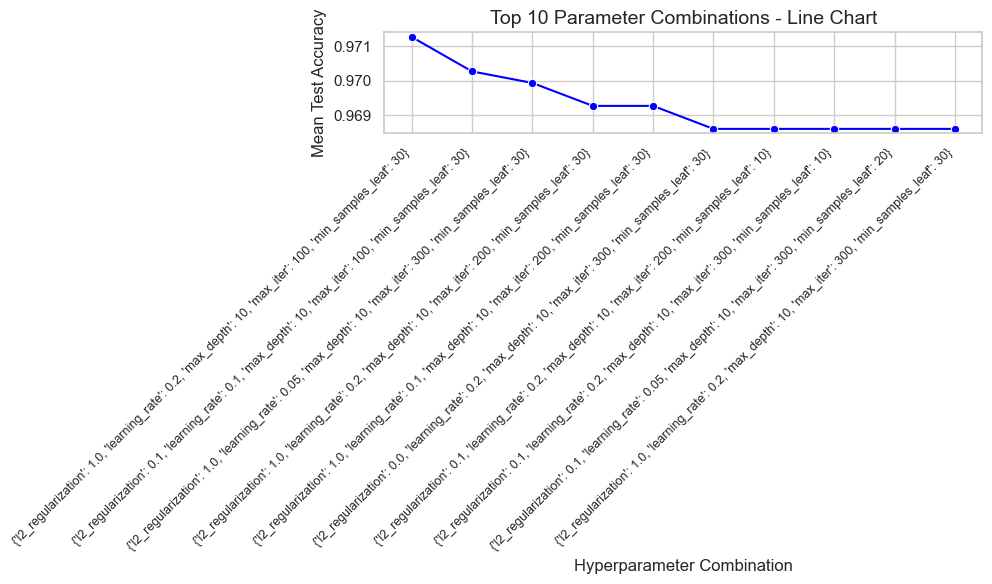
\includegraphics[width=0.9\linewidth]{Graph/hyper parament analysis of histgradient/hyperparameter_combination_line.png}
    \caption{Visual representation of Combination of best fit parameter}
    \label{fig:bestparameter}
\end{figure}
Fig~\ref{fig:bestparameter} displays the top 10 hyperparameter combinations based on mean test accuracy. The best performance (approx. 97.15\% accuracy) was achieved with specific combinations of parameters, while most top configurations shared a \texttt{max\_depth} of 10 and \texttt{min\_samples\_leaf} of 30.

On the other hand, the confusion matrix provides counts of True Positives (TP), True Negatives (TN), False Positives (FP), and False Negatives (FN). Minimizing FN (missed cases) is particularly important in medical contexts. \hyperref[tab:algorithm_metrics]{Table~\ref{tab:algorithm_metrics}} shows the confusion matrix counts for each algorithm.
\begin{table}
\centering
    \caption{Confusion Matrix' Metrics of Different Algorithms}
    \label{tab:algorithm_metrics}
\begin{tabular}{lrrrr}
        \toprule
        \textbf{Algorithm} & \textbf{TN} & \textbf{FP} & \textbf{FN} & \textbf{TP} \\
        \midrule
        LR & 274 & 65 & 84 & 326 \\
        NB & 306 & 43 & 68 & 332 \\
        DT(log-loss) & 312 & 27 & 20 & 390 \\
        KNN(Euclidean) & 330 & 19 & 26 & 374 \\
        SVM(RBF) & 334 & 15 & 7 & 393 \\
        RF & 337 & 12 & 18 & 382 \\
        HGBC & 343 & 6 & 10 & 390 \\
        \bottomrule
    \end{tabular}
\end{table}

\begin{figure}
    \centering
     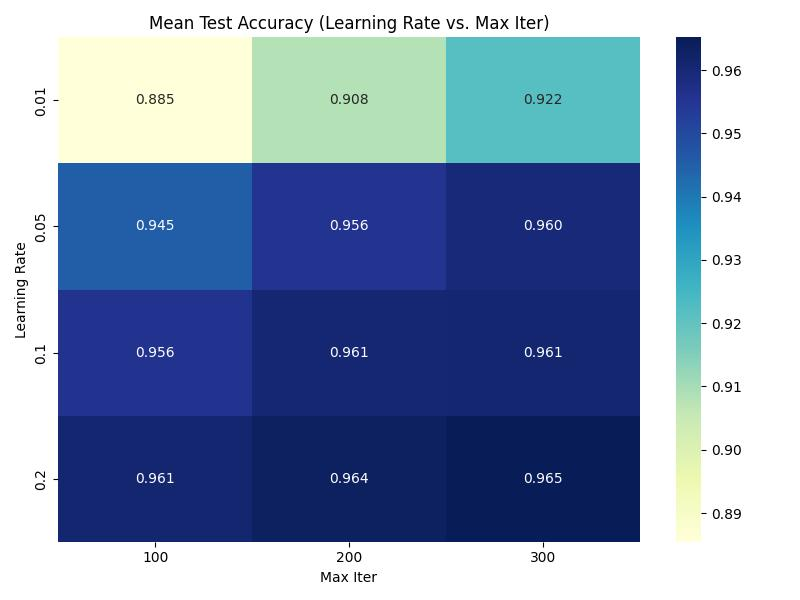
\includegraphics[width=0.6\linewidth]{best_accuracy.jpeg}
    \caption{\centering Heatmap}
    \label{fig:bestaccuracy} % Requires the caption package
\end{figure}

Fig~\ref{fig:bestaccuracy} shows a heatmap of mean test accuracy varying with \texttt{learning\_rate} and \texttt{max\_iter}. Accuracy generally increased with higher learning rates (peaking at 0.2) and increasing \texttt{max\_iter} (stabilizing around 300). The highest accuracy in this slice was achieved with a learning rate of 0.2 and max iterations of 300.

%\subsection{Evaluation Metrics}\label{sec:evalmetrics}
%
%Model performance was assessed using metrics derived from the confusion matrix, which summarizes prediction outcomes \cite{mahcine}.

%\begin{table}[ht]
%    \centering
%    \caption{Confusion Matrix Metrics of Different Algorithms}
%    \label{tab:algorithm_metrics}
%    \begin{tabular}{lrrrr}
%        \toprule
%        \textbf{Algorithm} & \textbf{TN} & \textbf{FP} & \textbf{FN} & \textbf{TP} \\
%        \midrule
%        LR & 274 & 65 & 84 & 326 \\
%        NB & 306 & 43 & 68 & 332 \\
%        DT(log-loss) & 312 & 27 & 20 & 390 \\
%        KNN(Euclidean) & 330 & 19 & 26 & 374 \\
%        SVM(RBF) & 334 & 15 & 7 & 393 \\
%        RF & 337 & 12 & 18 & 382 \\
%        HGBC & 343 & 6 & 10 & 390 \\
%        \bottomrule
%    \end{tabular}
%\end{table}

\subsection{Precision and Recall}\label{sec:precision_recall}
Precision (TP / (TP + FP)) and Recall (TP / (TP + FN)) are critical metrics for evaluating the model's ability to correctly identify positive cases and avoid false positives. Graphical representations are provided for illustration.
\FloatBarrier
\begin{minipage}{0.48\textwidth}
   \centering
    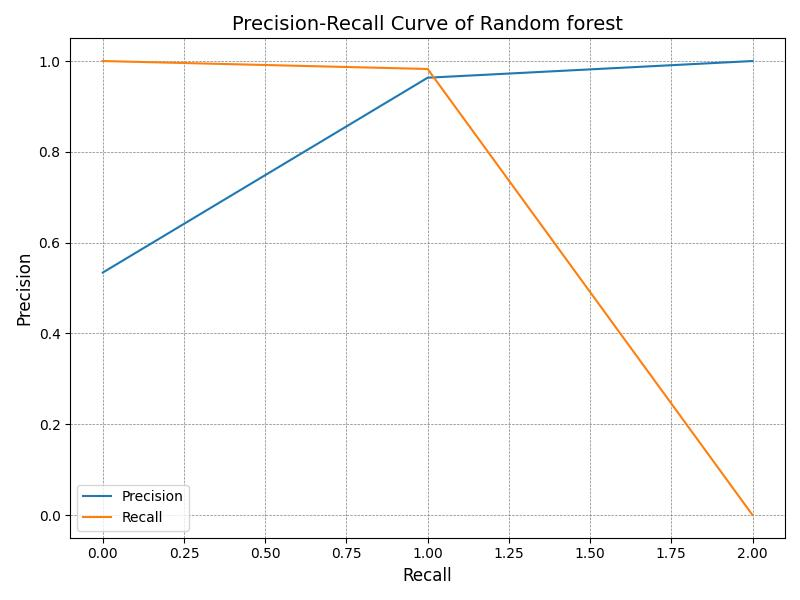
\includegraphics[width=0.9\linewidth]{Graph/precision and recall graph/pre_re_rf.jpeg}
    \captionof{figure}{Precision and Recall: RF}
    \label{fig:pre-re-rf}
\end{minipage}
\hfill % Adds horizontal space between minipages
   \begin{minipage}{0.48\textwidth}
    \centering
    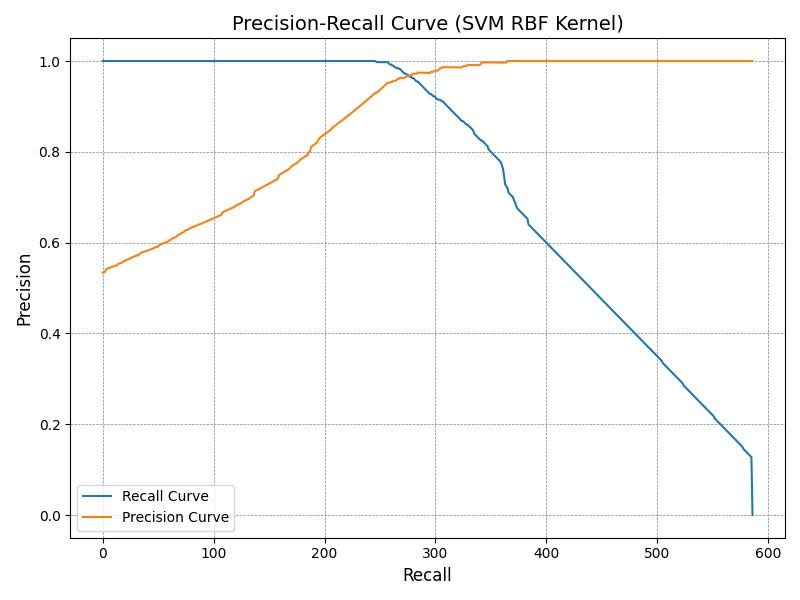
\includegraphics[width=0.9\linewidth]{Graph/precision and recall graph/pre_re_svm.jpeg}
    \captionof{figure}{Precision and Recall: SVF}
    \label{fig:pre-re-svm}
\end{minipage}
Precision and recall were visualized for Random Forest (\hyperref[Fig. 3]{Fig \ref{fig:pre-re-rf}}) and Support Vector Machine (\hyperref[Fig. 4]{Fig \ref{fig:pre-re-svm}}).

\subsection{Accuracy and F1 Score}\label{sec:f1score}
Accuracy is the proportion of correct predictions among all instances:
\begin{equation}
    \text{Accuracy} = \frac{\text{TP} + \text{TN}}{\text{TP} + \text{FP} + \text{TN} + \text{FN}}
    \label{eq:acc}
\end{equation}

The F1 Score is the harmonic mean of precision and recall, offering a balanced measure, especially useful for imbalanced datasets \cite{mahcine}.
\begin{equation}
    \text{F1 Score} = 2 \cdot \frac{\text{Precision} \cdot \text{Recall}}{\text{Precision} + \text{Recall}}
    \label{eq:f1}
\end{equation}

\begin{minipage}{0.49\textwidth}
    \centering
    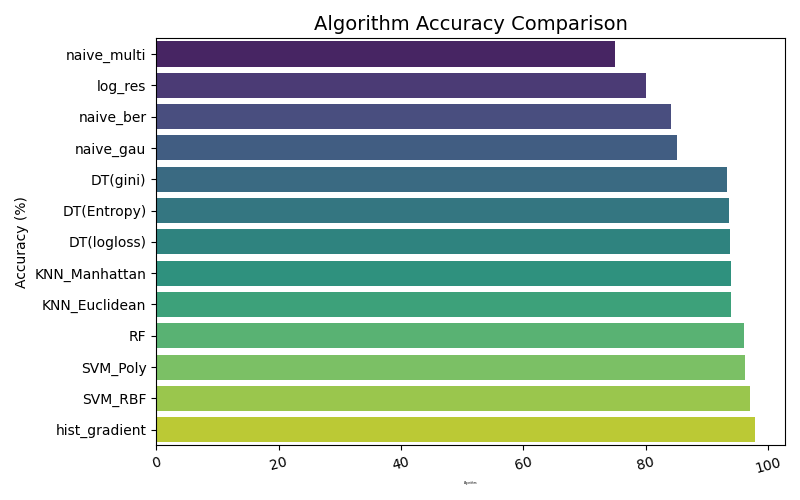
\includegraphics[width=0.9\linewidth]{accuracy.png}
    \captionof{figure}{\centering Accuracy of the different classification techniques}
    \label{fig:acc}
\end{minipage}
\hfill
\begin{minipage}{0.49\textwidth}
  \centering
    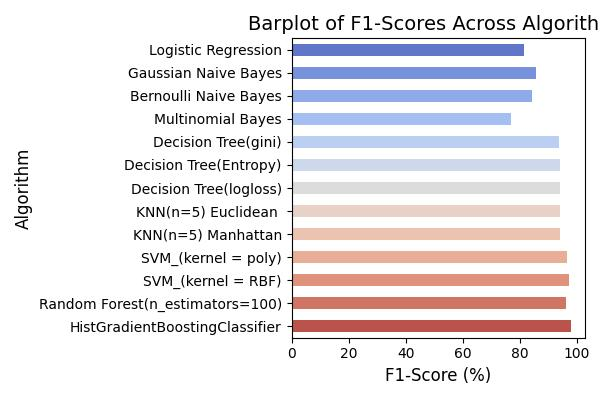
\includegraphics[width=0.9\linewidth]{Graph/DS/f1_score.jpeg}
    \captionof{figure}{\centering F1-score of all the classification models}
    \label{fig:f1_score}
\end{minipage}

\begin{table}[!ht]
    \centering
    \caption{Performance Matrix Including All Parameters}
    \renewcommand{\arraystretch}{1}
    \setlength{\tabcolsep}{1pt}
    \begin{tabular}{|c|l|c|c|c|c|}
        \hline
        \textbf{No.} & \textbf{Algorithms} & \textbf{Accuracy(\%)} & \textbf{Precision(\%)} & \textbf{Recall(\%)} & \textbf{F1-Score(\%)} \\
        \hline
          1  & Logistic Regression & 80.11 & 83.38 & 79.51 & 81.40 \\
          \hline
          2 & Naive Bayes & 85.18 & 88.53 & 83.00 & 85.68 \\
          \hline
          3 & Decision Tree & 93.72 & 93.53 & 95.12 & 94.32 \\
          \hline
          4 & k-nearest neighbor & 93.99 & 95.17 & 94.30 & 94.33 \\
          \hline
          5 & Support Vector Machine & 97.06 & 96.32 & 98.25 & 97.28 \\
          \hline
          6 & Random Forest & 95.99 & 96.95 & 95.50 & 96.22 \\
          \hline
          7 & HGBC & \textbf{97.86} & \textbf{98.48} & \textbf{97.50} & \textbf{97.90} \\
          \hline
    \end{tabular}
    \label{tab:Performance_Matrix}
\end{table}
The performance results based on accuracy, precision, recall, and F1-score are presented in \hyperref[tab:Performance_Matrix]{Table~\ref{tab:Performance_Matrix}}. The HGBC model demonstrated the highest accuracy (97.86\%), precision (98.48\%), recall (97.50\%), and F1-score (97.90\%). SVM also performed strongly with high accuracy (97.06\%) and particularly high recall (98.25\%). Ensemble methods like HGBC and Random Forest, along with SVM, were found to be well-suited for this predictive task. Hyperparameter tuning further optimized the HGBC model's performance.

\subsection{Comparison Study}\label{sec:results}
\begin{table}[ht!]
    \centering
    \caption{Comparison with Previous ASD Prediction Models}
    \renewcommand{\arraystretch}{1.3}
    \setlength{\tabcolsep}{6pt}
    \begin{tabular}{|p{5.5cm}|p{2.5cm}|c|c|c|c|}
        \hline
        \textbf{Study} & \textbf{Algorithm} & \textbf{Acc.} & \textbf{Prec.} & \textbf{Rec.} & \textbf{F1} \\
        \hline
        \multirow{3}{=}{A Comparison of Machine Learning Algorithms for the Surveillance of Autism Spectrum Disorder \cite{pmcid}} 
        & Naive Bayes & 73 & -- & -- & 78 \\
        & CVM & 87 & -- & -- & 83.6 \\
        & Random Forest & 87.1 & -- & -- & 86.8 \\
        \hline
        \multirow{3}{=}{An Evaluation of Machine Learning Approaches for Early Diagnosis of Autism Spectrum Disorder \cite{rasul2023evaluation}} 
        & Random Forest & 94 & 90.1 & 88.3 & -- \\
        & Naive Bayes & 85 & 84 & 81 & -- \\
        & SVM & 80 & 81 & 80 & -- \\
        \hline
        \multirow{3}{=}{Towards Equitable ASD Diagnostics: A Comparative Study of Machine and Deep Learning Models Using Behavioral and Facial Data \cite{aledhari2024equitable}} 
        & SVM & 89 & -- & -- & -- \\
        & KNN & 80 & -- & -- & -- \\
        & Gaussian NB & 81 & -- & -- & -- \\
        \hline
        \multirow{4}{=}{Machine Learning-Based Models for Early Stage Detection of Autism Spectrum Disorders \cite{8895818}} 
        & Naive Bayes & 96 & -- & -- & 97 \\
        & SVM & 85 & -- & -- & -- \\
        & KNN & 90 & -- & -- & -- \\
        & Random Forest & \textbf{99} & -- & -- & -- \\
        \hline
        \multirow{4}{=}{Detection of Autism Spectrum Disorder (ASD) in Children and Adults Using Machine Learning \cite{nature2023detection}} 
        & Logistic Regression & 97.15 & -- & -- & 98 \\
        & Naive Bayes & 94 & -- & -- & 96 \\
        & KNN & 90.52 & -- & -- & 93 \\
        & Random Forest & 81.52 & -- & -- & 88 \\
        \hline
    \end{tabular}
    \label{tab:Comparative_Studies}
\end{table}
Our approaches have been compared with some notable literary works done in the contemporaty space on the similar topics and a short hand comparison has been done in the Table \ref{tab:Comparative_Studies}.
As observed, our HGBC model surpasses most reported performances in previous works, particularly in terms of both accuracy (97.86\%) and F1-score (97.90\%). Notably, some studies reported higher individual values (e.g., Random Forest with 99\% in one case), but often under limited or imbalanced datasets.

Many prior works suffered from common issues such as class imbalance, lack of feature diversity, high dimensionality, noise, or overfitting. Our approach incorporated extensive pre-processing, balanced datasets, and hyperparameter tuning to mitigate these issues—thereby improving generalization and robustness of the model.

\subsection{Exploratory Data Analysis} \label{sec:data_analysis}
Exploratory Data Analysis (EDA) was conducted to understand the distribution of ASD traits across different demographic factors within the dataset.
\subsubsection{\textbf{Distribution Based on Ethnicity}}
\begin{figure}[ht!]
  \centering
    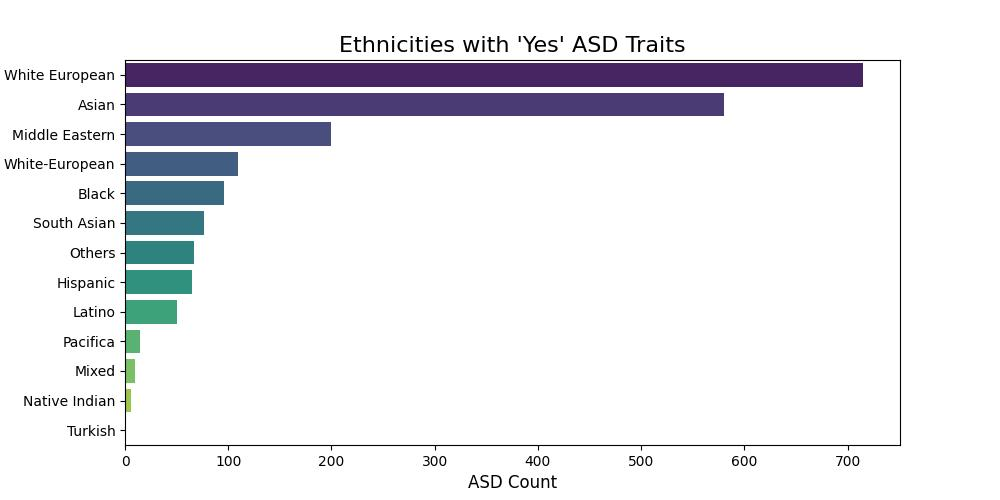
\includegraphics[width=0.9\linewidth]{Graph/EDA/Ethnicity_yes.jpeg}
    \captionof{figure}{The ethnics with the ASD traits as \enquote{YES}}
    \label{fig:ethni}
\end{figure}
ASD traits were found to be most prevalent in White Europeans within this dataset (\hyperref[fig:ethni]{Fig \ref{fig:ethni}}). This observation could be influenced by various factors, including genetic, social, environmental influences, and potentially higher awareness and access to diagnostic testing in these populations.
\subsubsection{Distribution Based on Sex:}
Analysis indicated that males exhibited ASD traits more frequently than females in this dataset (\hyperref[fig:gen]{Fig \ref{fig:gen}}). Hormonal differences, such as the influence of testosterone on brain development, are often considered as potential contributing factors to this observed gender disparity in ASD prevalence.

\begin{minipage}{0.49\textwidth}
    \centering
    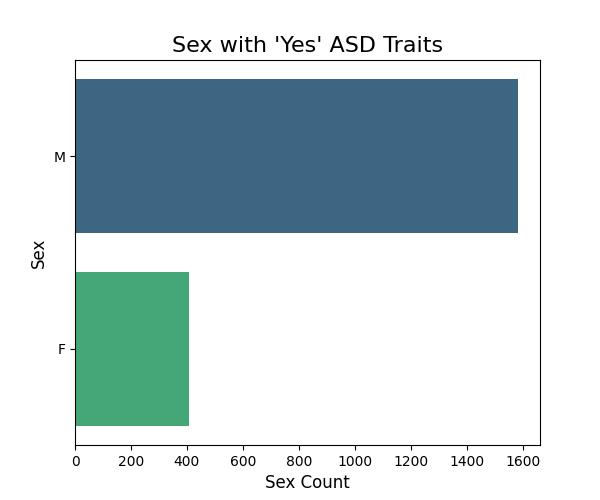
\includegraphics[width=0.99\linewidth]{Graph/EDA/sex.jpeg}
     \vspace{10pt}
    \captionof{figure}{\centering Gender distribution with ASD traits as \enquote{YES}}
    \label{fig:gen}
\end{minipage}
\hfill
\hfill
\begin{minipage}{0.49\textwidth}
    \centering
     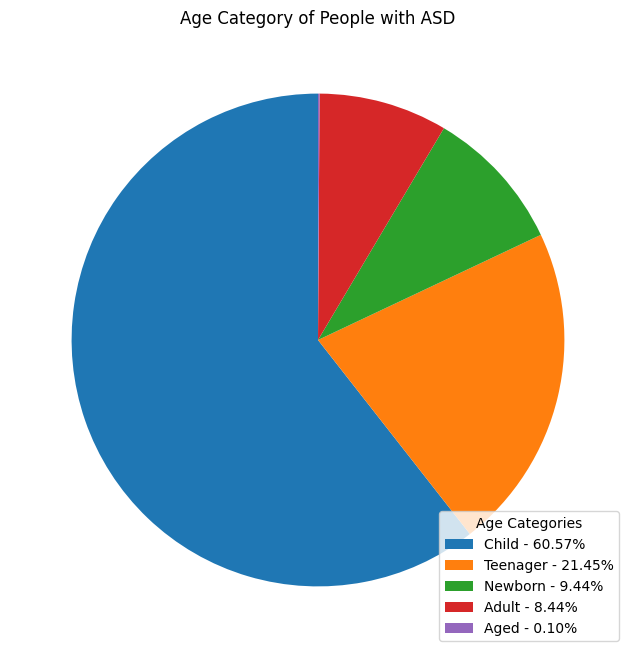
\includegraphics[width=0.9\linewidth]{Graph/EDA/age_chart.png}
    \captionof{figure}{\centering Age categories distribution of ASD traits:}
    \label{fig:age}
\end{minipage}

\subsubsection{Distribution Based on Age Category}
It was observed that ASD traits were most commonly reported in children, specifically affecting 60.57\% of individuals in the child age category (2-12 years) within the dataset (\hyperref[fig:age]{Fig \ref{fig:age}}). This highlights a period of significant susceptibility to exhibiting these traits.

%\begin{figure}[ht]
%    \centering
%    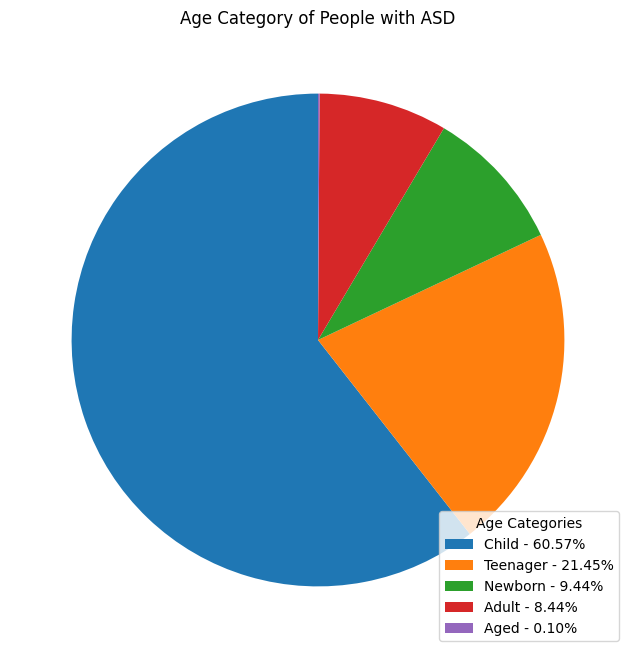
\includegraphics[width=0.6\linewidth]{Graph/EDA/age_chart.png}
%    \caption{Age categories distribution of ASD traits:}
%    \label{fig:age}
%\end{figure}
%
%\begin{table}[ht]
%    \centering
%    \caption{Age Category Traits in Percentage}
%    \vspace{0.8em}
%    \renewcommand{\arraystretch}{1.3} % Taller rows
%    \setlength{\tabcolsep}{20pt}     % Wider columns
%    \begin{tabular}{|c|c|}
%        \hline
%        \textbf{Age Category} & \textbf{Traits (\%)} \\
%        \hline
%        Newborn & 9.44\% \\
%        \hline
%        Child & 60.57\% \\
%        \hline
%        Teenager & 21.45\% \\
%        \hline
%        Adult & 8.44\% \\
%        \hline
%        Aged & 0.10\% \\
%        \hline
%    \end{tabular}
%    \label{tab:age-category}
%\end{table}

\subsubsection{Distribution Based on Genetics}
\begin{figure}[ht!]
    \centering
    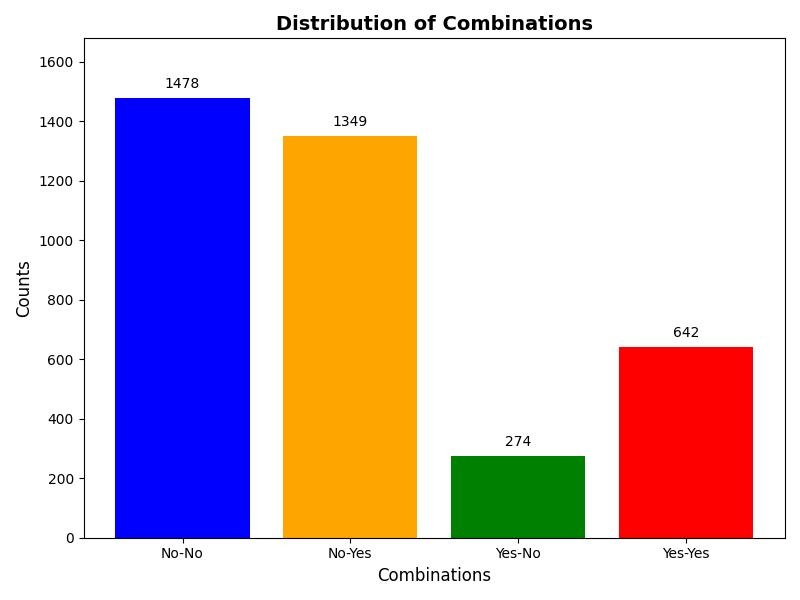
\includegraphics[width=0.6\linewidth]{Graph/EDA/fam_mem.jpeg}
    \caption{\centering The distribution of family member traits of ASD}
    \label{fig:genetics}
\end{figure}
Analysis of family history within the dataset suggested that, for most individuals with ASD traits, other family members did not have diagnosed ASD traits (\hyperref[fig:genetics]{Fig \ref{fig:genetics}}). While genetics are known to play a role in ASD, this dataset suggests that non-genetic factors, such as environmental influences or early social experiences, may also contribute significantly to trait development.

\section{Conclusion}
\label{sec:conclusion}
This study successfully demonstrated the potential of supervised machine learning in predicting ASD traits using a quantitative dataset. Various classification algorithms were evaluated, with the HGBC emerging as the most effective model. HGBC achieved the highest accuracy of 97.86\%, along with superior precision (98.48\%), recall (97.50\%), and F1-score (97.90\%), indicating its strong capability in correctly identifying individuals with ASD traits while minimizing false positives. Support Vector Machine and Random Forest models also showed commendable performance.

Exploratory Data Analysis provided valuable insights into the dataset's characteristics and the distribution of ASD traits. Key findings included the high prevalence of ASD traits in children (60.57\% in the child age category), the higher occurrence in males compared to females, and observations regarding ethnicity and family history, suggesting a multifactorial influence on trait manifestation.

The results highlight HGBC's potential as a valuable tool to complement traditional clinical assessments for early ASD detection. Improved early screening could facilitate timely interventions, which are known to enhance outcomes for individuals with ASD. Further advancements in machine learning techniques and the availability of more extensive datasets are expected to further improve prediction performance. The integration of these technologies into clinical workflows holds promise for developing more scalable and efficient ASD screening programs. This research represents a significant step in applying computational methods to address a critical public health challenge. Future work could involve validating the models on larger, more diverse datasets and exploring explainable AI techniques to understand the model's decision-making process better, which could further increase trust and utility in clinical settings.

\begin{thebibliography}{99}
\bibitem{1in31}
Centers for Disease Control and Prevention (2024) Autism Spectrum Disorder (ASD) - Data and Statistics. Accessed: 2025-04-20.

\bibitem{ini3}
Lord, C., Rutter, M. and Le Couteur, A. (1994) Autism Diagnostic Interview-Revised: A revised version of a diagnostic interview for caregivers of individuals with possible pervasive developmental disorders. \emph{Journal of Autism and Developmental Disorders} \textbf{24}(5), 659--685. doi:10.1007/BF02172145

\bibitem{bib12}
Stevens, E., Dixon, D. R., Novack, M. N., Granpeesheh, D., Smith, T. and Linstead, E. (2019) Identification and analysis of behavioral phenotypes in autism spectrum disorder via unsupervised machine learning. \emph{International Journal of Medical Informatics} \textbf{129}, 29--36. doi:10.1016/j.ijmedinf.2019.05.006

\bibitem{bib14}
Prasad, V., Sriramakrishnan, G.V. and Diana Jeba Jingle, I. (2023) Autism spectrum disorder detection using brain MRI image enabled deep learning with hybrid sewing training optimization. \emph{Signal, Image and Video Processing} \textbf{17}, 4001--4008. doi:10.1007/s11760-023-02630-y

\bibitem{parlett2023applications}
Parlett-Pelleriti, C. M., Stevens, E., Dixon, D. et al. (2023) Applications of Unsupervised Machine Learning in Autism Spectrum Disorder Research: a Review. \emph{Review Journal of Autism and Developmental Disorders} \textbf{10}, 406--421. doi:10.1007/s40489-021-00299-y

\bibitem{nogay2020machine}
Nogay, H. S. and Adeli, H. (2020) Machine learning (ML) for the diagnosis of autism spectrum disorder (ASD) using brain imaging. \emph{Reviews in the Neurosciences} \textbf{31}(8), 825--841. doi:10.1515/revneuro-2020-0043

\bibitem{bib3}
Parlett-Pelleriti, C. M., Stevens, E., Dixon, D. et al. (2023) Applications of Unsupervised Machine Learning in Autism Spectrum Disorder Research: a Review. \emph{Review Journal of Autism and Developmental Disorders} \textbf{10}, 406--421. doi:10.1007/s40489-021-00299-y

\bibitem{bib4}
Vakadkar, K., Purkayastha, D. and Krishnan, D. (2021) Detection of Autism Spectrum Disorder in Children Using Machine Learning Techniques. \emph{SN Computer Science} \textbf{2}, 386. doi:10.1007/s42979-021-00776-5

\bibitem{bib5}
Alves, C. L., Toutain, T. G. L. d. O., de Carvalho Aguiar, P. et al. (2023) Diagnosis of Autism Spectrum Disorder Based on Functional Brain Networks and Machine Learning. \emph{Scientific Reports} \textbf{13}, 8072. doi:10.1038/s41598-023-34650-6

\bibitem{bib6}
Mellema, C. J., Nguyen, K. P., Treacher, A. et al. (2022) Reproducible Neuroimaging Features for Diagnosis of Autism Spectrum Disorder with Machine Learning. \emph{Scientific Reports} \textbf{12}, 3057. doi:10.1038/s41598-022-06459-2

\bibitem{bib7}
Zhou, Y., Jia, G., Ren, Y. et al. (2024) Advancing ASD Identification with Neuroimaging: A Novel GARL Methodology Integrating Deep Q-Learning and Generative Adversarial Networks. \emph{BMC Medical Imaging} \textbf{24}, 186. doi:10.1186/s12880-024-01360-y

\bibitem{bib8}
Rajagopalan, S. S., Zhang, Y. and Yahia, A. (2024) [Title not provided -- please update with article title]. \emph{JAMA Network Open} \textbf{7}(8), e2429229. doi:10.1001/jamanetworkopen.2024.29229

\bibitem{bib10}
Jaradat, A. S., Wedyan, M., Alomari, S. and Barhoush, M. M. (2025) Using Machine Learning to Diagnose Autism Based on Eye Tracking Technology. \emph{Diagnostics} \textbf{15}(1), 66. doi:10.3390/diagnostics15010066

\bibitem{bib13}
Eslami, T. and Saeed, F. (2021) Explainable and scalable machine learning algorithms for detection of autism spectrum disorder using fMRI data. In El-Baz, A. S. and Suri, J. S. (eds.) \emph{Neural Engineering Techniques for Autism Spectrum Disorder}, pages 39-54. Academic Press. doi:10.1016/B978-0-12-822822-7.00004-1

\bibitem{datapre}
Kotsiantis, S., Kanellopoulos, D. and Pintelas, P. (2006) Data Preprocessing for Supervised Learning. \emph{International Journal of Computer Science} \textbf{1}, 111--117.

\bibitem{hosmer2000applied}
Hosmer, D. W. and Lemeshow, S. (2000) \emph{Applied Logistic Regression}. 2nd edition. Wiley, New York.

\bibitem{decision}
Mienye, I. D. and Jere, N. (2024) A Survey of Decision Trees: Concepts, Algorithms, and Applications. \emph{IEEE Access} \textbf{12}, 86716--86727. doi:10.1109/ACCESS.2024.3416838

\bibitem{KNN}
Taunk, K., De, S., Verma, S. and Swetapadma, A. (2019) A Brief Review of Nearest Neighbor Algorithm for Learning and Classification. In \emph{2019 International Conference on Intelligent Computing and Control Systems (ICCS)}, pages 1255-1260. doi:10.1109/ICCS45141.2019.9065747

\bibitem{naive}
Chen, H., Hu, S., Hua, R. et al. (2021) Improved naive Bayes classification algorithm for traffic risk management. \emph{EURASIP J. Adv. Signal Process} \textbf{2021}(30).

\bibitem{rand}
Breiman, L. (2001) Random Forests. \emph{Machine Learning} \textbf{45}(1), 5--32. doi:10.1023/A:1010933404324

\bibitem{svm}
Hearst, M. A., Dumais, S. T., Osuna, E., Platt, J. and Scholkopf, B. (1998) Support vector machines. \emph{IEEE Intelligent Systems and their Applications} \textbf{13}(4), 18--28. doi:10.1109/5254.708428

\bibitem{hist}
Maftoun, M., Shadkam, N., Komamardakhi, S. S. S., Mansor, Z. and Joloudari, J. H. (2024) Malicious URL Detection using optimized Hist Gradient Boosting Classifier based on grid search method. arXiv preprint arXiv:2404.13050.

\bibitem{para}
Ilemobayo, J., Durodola, O., Alade, O., Awotunde, O., Adewumi, T., Falana, O., Ogungbire, A., Osinuga, A., Ogunbiyi, D., Odezuligbo, I., Edu, O. and Ifeanyi, A. (2024) Hyperparameter Tuning in Machine Learning: A Comprehensive Review. \emph{Journal of Engineering Research and Reports} \textbf{26}, 388--395. doi:10.9734/jerr/2024/v26i61188

\bibitem{mahcine}
Bishop, C. M. (2006) \emph{Pattern Recognition and Machine Learning}. Springer, New York, NY.

\bibitem{pmcid}
Lee, Scott H. and Maenner, Matthew J. and Heilig, Charles M. \emph{A Comparison of Machine Learning Algorithms for the Surveillance of Autism Spectrum Disorder} \textbf{Proceedings of IJ-CSE (Atlantis Press)} 10.2991/aer.k.201124.028

\bibitem{rasul2023evaluation}
Rasul, Rownak Ara and Saha, Promy and Bala, Diponkor and Karim, S.M. Rakib Ul and Abdullah, Md. Ibrahim and Saha, Bishwajit
\emph{An Evaluation of Machine Learning Approaches for Early Diagnosis of Autism Spectrum Disorder}

\bibitem{aledhari2024equitable}
Aledhari, Mohammed and Rahouti, Mohamed and Alfatemi, Ali
\emph{Towards Equitable ASD Diagnostics: A Comparative Study of Machine and Deep Learning Models Using Behavioral and Facial Data}

\bibitem{8895818}
Akter, Tania and Shahriare Satu, Md. and Khan, Md. Imran and Ali, Mohammad Hanif and Uddin, Shahadat and Lió, Pietro and Quinn, Julian M. W. and Moni, Mohammad Ali
\emph{Machine Learning-Based Models for Early Stage Detection of Autism Spectrum Disorders}
\textbf{IEEE Access} 2019 166509-166527

\bibitem{nature2023detection}
Muhammad Shoaib Farooq, Rabia Tehseen, Maidah Sabir \& Zabihullah Atal
\emph{Detection of Autism Spectrum Disorder (ASD) in Children and Adults Using Machine Learning}
\textbf{Scientific Reports (Nature)} 2023

\end{thebibliography}
\end{document}